% Chapter Template

\chapter{Modelado dinámico} % Main chapter title

\label{DINAMICA} % Change X to a consecutive number; for referencing this chapter elsewhere, use \ref{ChapterX}

%----------------------------------------------------------------------------------------
%	SECTION 1
%----------------------------------------------------------------------------------------

\section{Dinámica de las comunidades mutualistas}

Lorem ipsum dolor sit amet, consectetur adipiscing elit. Aliquam ultricies lacinia euismod. Nam tempus risus in dolor rhoncus in interdum enim tincidunt. Donec vel nunc neque. In condimentum ullamcorper quam non consequat. Fusce sagittis tempor feugiat. Fusce magna erat, molestie eu convallis ut, tempus sed arcu. Quisque molestie, ante a tincidunt ullamcorper, sapien enim dignissim lacus, in semper nibh erat lobortis purus. Integer dapibus ligula ac risus convallis pellentesque .

%-----------------------------------
%	SUBSECTION 1
%-----------------------------------
\subsection{Modelos de población}

El uso de modelos cuantitativos en el estudio de la dinámica de poblaciones fue una de las primeras aplicaciones de las matemáticas en el campo de la biología, con antecedentes tan remotos como Fibonacci y Malthus. Todo modelo supone una descripción simplificada del fenómeno que se quiere estudiar y las formulaciones clásicas, como la de crecimiento de Verhulst o la de interacción presa-depredador de Lotka-Volterra  resultaban muy atractivas por su sencillez, aunque limitadas a la hora de aplicarlas a escenarios reales. Los modelos se fueron refinando, pero el paradigma se mantuvo hasta finales del siglo XX

\section{Modelo con capacidad de carga constante}

Nunc posuere quam at lectus tristique eu ultrices augue venenatis. Vestibulum ante ipsum primis in faucibus orci luctus et ultrices posuere cubilia Curae; Aliquam erat volutpat. Vivamus sodales tortor eget quam adipiscing in vulputate ante ullamcorper. Sed eros ante, lacinia et sollicitudin et, aliquam sit amet augue. In hac habitasse platea dictumst.

Probando fórmulas. Como dice la fórmula \ref{myeq1}...

\begin{align}
\displaystyle &\frac{dN}{dt}=N\, \left(a-b \,P\right), \nonumber\\
\displaystyle &\frac{dP}{dt}=P\, \left(c\, N-d\right) , 
\label{myeq1}
\end{align}

Otra fórmula más. Como se demuestra en \ref{eq:reffs_2especies}...
\begin{align}
A = & \, r_{1}+ b_{12}\, {N_2^a}^0 - (\alpha_{1}+ c_{1} \, b_{12}\, {N_{2}^a}^0) \, {N_1^p}^0 , \nonumber\\
-B = &\, r_{2} + b_{21} \, {N_{1}^p}^0-(\alpha_{2}+ c_{2}\,  b_{21}\, {N_{1}^p}^0)\,  {N_{2}^a}^0 .
\label{eq:reffs_2especies}
\end{align}

\subsection{Análisis de estabilidad}

Nunc posuere quam at lectus tristique eu ultrices augue venenatis. Vestibulum ante ipsum primis in faucibus orci luctus et ultrices posuere cubilia Curae; Aliquam erat volutpat. Vivamus sodales tortor eget quam adipiscing in vulputate ante ullamcorper. Sed eros ante, lacinia et sollicitudin et, aliquam sit amet augue. In hac habitasse platea dictumst.

\clearpage
\section{Modelo con saturación del beneficio}

La hipótesis de partida es que el mutualismo incrementa a tasa intrínseca de crecimiento de las especies. Esta suposición se basa en observaciones según las cuales la variación de la tasa de crecimiento de las poblaciones (o la fertilidad) tienen una alta correlación con la disponiblidad de recursos \cite{stenseth1998,krebs2002,rueness2003,tyler2008,jones2008}. En este contexto los recursos son las interacciones mutualistas. Supongamos que la comunidad está compuesta por $n_a$ especies de animales, con poblaciones$\{N_{i}^a\}$, y $n_p$ especies de plantas con poblaciones $\{N_{j}^p\}$. El beneficio mutualista entre las especies $i$  de una clase y $j$ de la otra se representa con el elemento $b_{ij}$ de la matriz de interacción. Debe tenerse en cuenta que las matrices no son necesariamente simétricas, y que la intensidad del beneficio de la interacción no es el mismo en ambos sentidos. Para una especie animal $i$, escribimos su tasa de de crecimiento como
\begin{align}
r_{i} = r_{i}^{0} + \sum_{k=1}^{n_{p}} b_{ik}\, N^{p}_k
\label{eq:expr}
\end{align}
En esta expresión, $r_{i}^{0}$ es la tasa de crecimiento vegetativo. Para impedir un crecimiento ilimitado de dicha tasa, el efecto del mutualismo tiene que saturar en cierto punto.

Siguiendo la idea de Velhurst, proponemos un modelo en el que el término de fricción $\alpha_i$ depende también de la intensidad de la interacción mutualista. La traducción biológica de esta idea es que a partir de un determinado nivel el aumento de individuos de la especie mutualista no aporta beneficio adicional. Imaginemos una especie de polinizadores y una planta de la que obtiene alimento en forma de néctar. Si la población de plantas crece sin medida, llegará un momento en que los insectos no podrán libar todo el néctar producido. Para mantener el modelo simple, suponemos que el efecto del mutualismo sobre $\alpha$ es proporcional al beneficio. 
\begin{align}
\alpha_i = \alpha_{i}^{0}+ c_{i} \sum_{k=1}^{n_{p}} b_{ik}\, N^{p}_k 
\stepcounter{equation}\tag{\theequation}
\label{eq:alphavariable}
\end{align}
El término $c_{i}$ es el coeficiente de proporcionalidad. Las expresiones para las plantas son similares con el sumatorio sobre las especies de animales. Para simplificar la notación, eliminaremos los ceros de $\alpha_{i}^{0}$ y $r_{i}^{0}$ allí donde no haya confusión posible. Bajo estas suposiciones la dinámica del modelo propuesto está gobernada por el siguiente juego de ecuaciones:

\begin{theo} 
Modelo de dinámica mutualista con saturación de beneficio.
\begin{align*}
\frac{1}{N^{a}_{i}}\frac{dN^{a}_{i}}{dt} = r_{i}+ \sum_{k=1}^{n_{p}} b_{ik}\, N^{p}_k - \left( \alpha_{i}+ c_{i} \sum_{k=1}^{n_{p}} b_{ik}\, N^{p}_k \right) N^{a}_{i} \nonumber\\
\frac{1}{N^{p}_{j}}\frac{dN^{p}_{j}}{dt} = r_{j}+ \sum_{\ell=1}^{n_{a}} b_{j\ell}\, N^{a}_\ell - \left( \alpha_{j}+ c_{j} \sum_{\ell=1}^{n_{a}} b_{j\ell}\, N^{a}_\ell \right) N^{p}_{j}
\stepcounter{equation}\tag{\theequation}\label{eq:DINAMICA_modeloralphaconmut}
\end{align*}
\end{theo}


Las expresiones en el lado derecho de las igualdades se pueden interpretar como \textit{tasas de crecimiento efectivas}. Como vamos a usar este concepto más adelante, es importante definirlo de forma explícita.

\begin{theo} 
Tasa de crecimiemto eficaz de la especie animal $i$.
\begin{equation}
r_{ef,i} = r_{i} + \sum_{k=1}^{n_{p}} b_{ik}\, N^{p}_k - \left( \alpha_{i}+ c_{i} \sum_{k=1}^{n_{p}} b_{ik}\, N^{p}_k \right) N^{a}_{i}
\label{eq:DINAMICA_effrate}
\end{equation}
\end{theo}

Las tasas efectivas de las especies de plantas se definen de forma similar sustituyendo $a$ por $p$. Las \textit{capacidades de carga} del sistema son los puntos fijos distintos de cero de las ecuaciones \ref{eq:DINAMICA_modeloralphaconmut}. Es sencillo ver que en ausencia de mutualismo $K_i = r_i/\alpha_i$ para la especie $i$. Por el contrario, en presencia de mutualismo muy intenso, $K_i$ tiende a $1/c_{i}$. El papel de la constante de proporcionalidad $c_i$ es, por tanto, limitar la población máxima de la especie $i$ cuando $c_{i} \sum_{k=1}^{n_p} b_{ik} \, N^p_{k} \gg \alpha_{i}$. 

Consideramos que este modelo podría resultar también válido para otro tipo de interacciones ecológicas en las que todos los términos $b_{ik}$ son positivos, como el comensalismo Commensalism ($b_{ij}=0, b_{ji}>0)$ y el antagonismo ($b_{mn}>0,b_{nm}<0$). 

\subsection{Análisis de estabilidad para dos especies}

Por simplicidad empezamos con la comunidad mutualista más sencilla, formada por una especie de cada clase, para la cual podemos obtener resultados análiticos completos. Sea la planta la especie que designamos con el índice $1$ y el animal la representada como $2$. El modelo \ref{eq:DINAMICA_modeloralphaconmut} se reduce a:

\begin{align}
\frac{dN^p_{1}}{dt} = \left( r_{1}+ b_{12}\, N^a_{2}\right) \ N^p_{1} - \left(\alpha_{1}+ c_{1} \, b_{12} \, N^a_{2} \right) {N^p_{1}}^2 ,\nonumber\\ 
\frac{dN^a_{2}}{dt} = \left( r_{2}+ b_{21}\, N^p_{1}\right)N^a_{2} - \left(\alpha_{2}+ c_{2} \, b_{21}\, N^p_{1} \right) {N^a_{2}}^2 .
\stepcounter{equation}\tag{\theequation}\label{eq:DINAMICA_dos_especies}
\end{align}

La figura \ref{DINAMICA_diagram} representa varios diagramas de flujo del sistema con distintas configuraciones de los parámetros.

\begin{figure*}
\centering
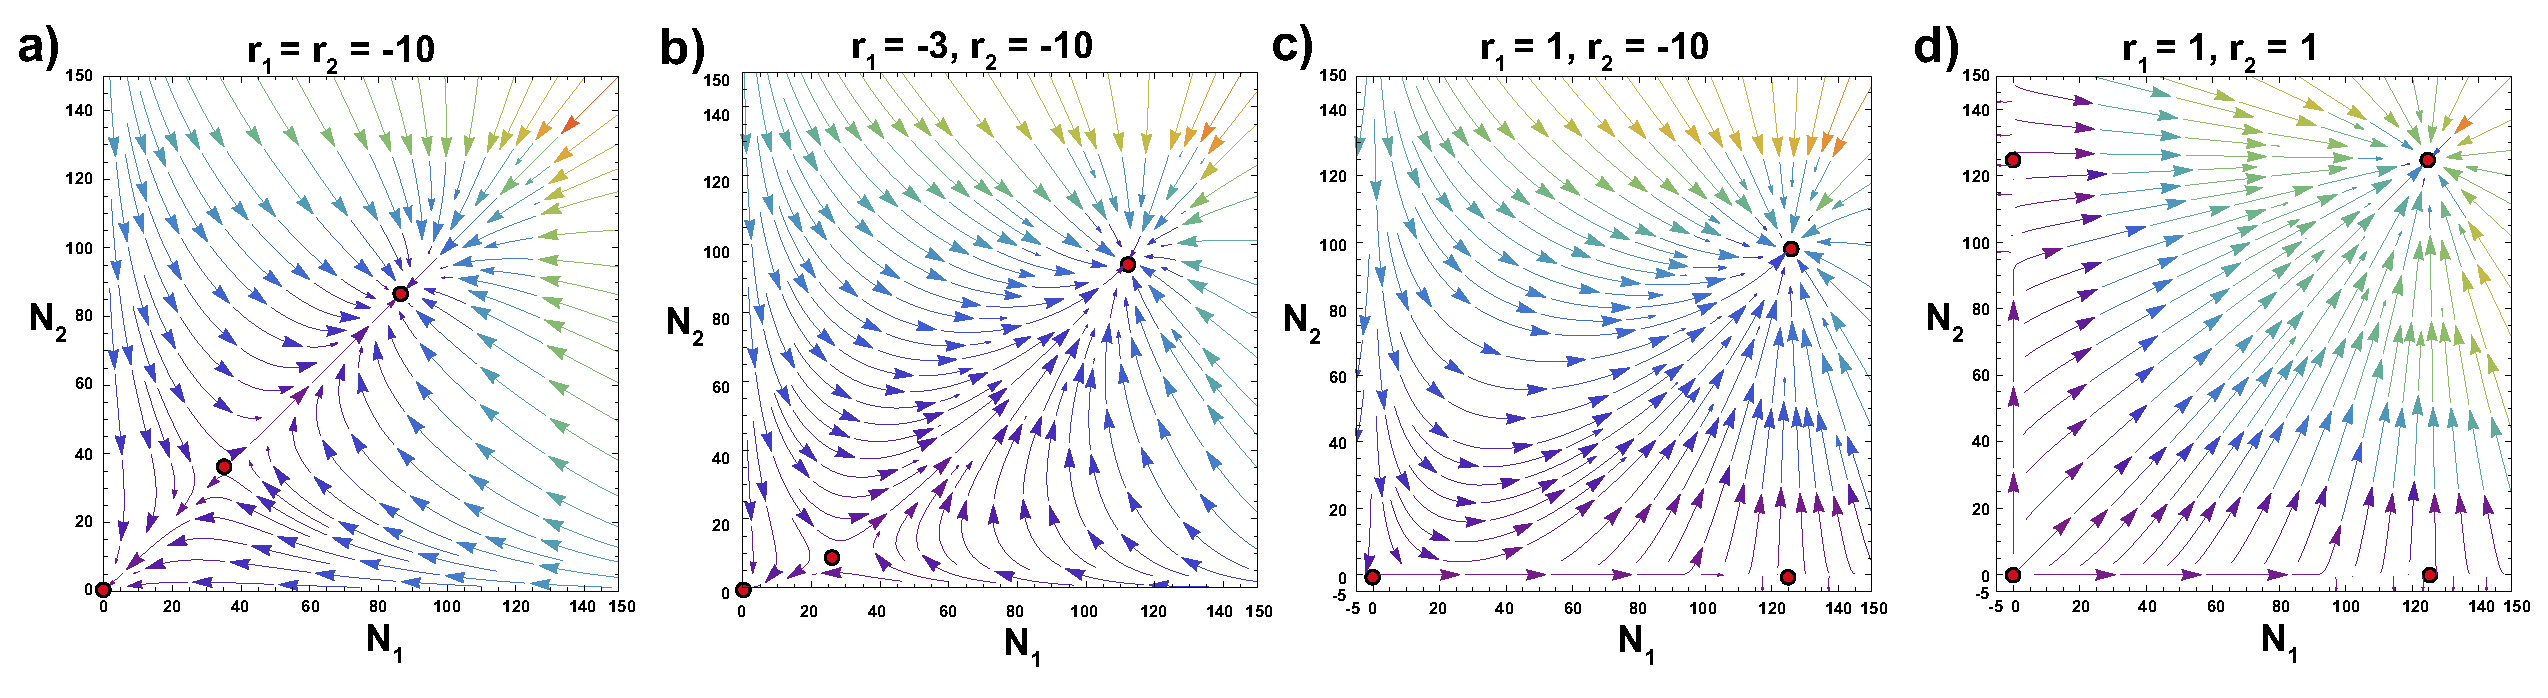
\includegraphics[scale=0.35]{DINAMICA_Figure1h.eps}
\caption {Diagrma de flujo de la dinámica de una comunidad de dos especies según el modelo de ecuaciones \ref{eq:DINAMICA_dos_especies}. Los puntos fijos se han resaltado como círculos de color rojo. El color de las flechas indica la intensidad del flujo. Las cuatro imágenes corresponden a diferentes valores para las tases intrínsecas de crecimimento. El resto de parámetros mantiene los mismos valores en los cuatro casos: $\alpha_1 = \alpha_2 = 0.008$, $b_{12} = b_{21} = 0.4$ and $c_1 = c_2 = 0.008$. El mutualismo es obligatorio en a) y b), aunque en diferente grado en el segundo diagrama. Es obligatorio para la especie 2 es c), mientras que la especie 1 podría sobrevivir sin la 2. En d) el mutualismo es facultativo para ambas especies.}
\label{DINAMICA_diagram}
\end{figure*}

Para encontrar los puntos fijos del sistema hacemos $\frac{dN^p_{1}}{dt} = \frac{dN^a_{2}}{dt} = 0$. El primero y más obvio, corresponde a la extinción total $({N^p_{1}}^*,{N^a_{2}}^*) = (0,0)$ con independencia del valor de los parámetros. Si cualquiera de las tasas de crecimiento intrínseco $r_1$, $r_2$ es positiva, entonces encontramos puntos fijos adicionales que aparecen por extinciones parciales. La dinámica de la población superviviente, con $r$ positivo, sigue en tal caso una ecuación logística como se deduce de la expresión \ref{eq:DINAMICA_dos_especies}. En consecuencia, su población tenderá a la capacidad de carga sin mutualismo ya sea $K_1 = r_1/\alpha_1$ o $K_2 = r_2/\alpha_2$. Las extinciones se producen en los puntos fijos $(K_1,0)$ o $(0,K_2)$, o en ambos si el mutualismo es facultativo solo para la especie $1$ ($r_1 >0$), solo para la especie dos $2$ ($r_2 >0$) (figura \ref{DINAMICA_diagram}c) o para las dos ($r_1>0$ y $r_2 >0$) (figura \ref{DINAMICA_diagram}d). 

Además de los puntos fijos correspondientes a extinciones, aparecen otros no triviales cuando se cumple la condición $r_{ef,i} = r_{ef,j} = 0$. Para dichos puntos se verifica que: 
\begin{align}
{N^p_{1}}^* = \frac{ r_{1}+ b_{12} \, {N^a_{2}}^* }{\alpha_{1}+ c_{1}\, b_{12}\, {N^a_{2}}^* } , \nonumber\\ 
{N^a_{2}}^* = \frac{ r_{2}+ b_{21}\, {N^p_{1}}^* }{\alpha_{2}+ c_{2} \, b_{21}\, {N^p_{1}}^* } .
\label{eq:DINAMICA_puntosfijos}
\end{align}

Sustituyendo la expresión de ${N^{a}_2}^*$ en la ecuación superior, encontramos que ${N^p_1}^*$ es la solución de una ecuación cuadrática en los puntos fijos: 
\begin{equation}
A\, {{N^p_1}^*}^2 + B \, {N^p_1}^* + C=0 ,
\label{eq:DINAMICA_quadra}
\end{equation}

Los coeficientes $A$, $B$ y $C$ valen:

\begin{align}
\displaystyle A &= c_{2}\, b_{21}\, \alpha_{1}+c_{1}\, b_{12}\, b_{21} , \nonumber \\
\displaystyle B &= \alpha_{1}\, \alpha_{2}+ c_{1}\, b_{12}\, r_{2} - c_{2}\, b_{21}\, r_{1} - b_{12}\, b_{21} ,\nonumber\\
\displaystyle C &= - r _{1}\, \alpha_{2} - b_{12}\, r_{2} .
\label{eq:DINAMICA_puntos_n1}
\end{align}

Los puntos fijos para ${N^a_2}^*$ se encuentran sustituyendo ${N^p_1}^*$ en la expresión inferior de la ecuación \ref{eq:DINAMICA_puntosfijos}. Aparecen distintos escenarios dependiendo de las soluciones de la ecuación \ref{eq:DINAMICA_quadra}:

\begin{enumerate}
\item Ambas raíces complejas. No hay puntos fijos que no supongan extinciones.
\item Una sola raíz real. Es un punto de bifuración de la dinámica del sistema. Las soluciones son reales pero degeneradas. En este caso existe un único punto fijo aparte de los de extinción. El estado final del sistema depende de la estabilidad de dicho punto. Sin embargo, lo más probable es que las poblaciones terminen extinguiéndose.
\item Dos raíces reales. La situación es similar a la representada en la imagen de la izquierda de la figura \ref{DINAMICA_diagram}. Hay dos puntos fijos no triviales, típicamente uno estable y un \textit{saddle} sobre la divisoria de las dos cuencas de atracción. La posición de este segundo punto depende de la extensión de la cuenca de extinción y, por tanto, de la resistencia del sistema ante perturbaciones externas. Lo denominamos \textit{umbral de extinción} y su valor lo representamos como$({N_{1}^{p}}^\bullet,{N_{2}^{a}}^\bullet)$.
\end{enumerate}

Para estudiar la estabilidad lineal de los puntos fijos, expandimos las ecuaciones \ref{eq:DINAMICA_dos_especies} en serie de Taylor en torno a ellos y calculamos el jacobiano del sistema (ver los detalles en el anexo....). Si los autovalores son negativos, el punto fijo es estable. En caso contrario, puede ser un \textit{saddle} si uno es positivo y otro negativo o inestable si ambos son negativos. Comenzando por la extinción total, el jacobiano puede escribirse como: 
\begin{equation}
J = \left(
\begin{array}{ll}
r_{1}   & 0 \\
0 & r_{2} 
\end{array}
\right) .\stepcounter{equation}\tag{\theequation}\label{eq:J00}
\end{equation}

Lo autovalores son $\lambda_{1,2} = r_{1,2}$, lo que indica que el punto de extinción es linealmente estable bajo la hipótesis de que $r_{1}<0$ y $r_{2}<0$; es decir, ambas especies dependen del mutualismo para sobrevivir. La extinción total tiene una cuenca de atracción para los distintos valores de las poblaciones. Si el sistema entra en ella, el único destino posible es la destrucción de la comunidad.

Por el contrario, si el mutualismo es facultativo para una o ambas especies, la extinción total se convierte en un \textit{saddle} o en un punto inestable. No obstante, pueden aparecer otros dos puntos fijos correspondientes a extinciones parciales. En estas circunstancias, la condición de estabilidad para $(r_1/\alpha_1, 0)$ es que $r_{1}>0$ y $r_{2}<-b_{21}\, r_{1}/\alpha_{1}$. Análogamente, $(r_1/\alpha_1, 0)$ es estable si y solo si  $r_{2}>0$ y $r_{1}<-b_{12}\, r_{2}/\alpha_{2}$.
El mismo análisis para los restantes casos de puntos fijos no triviales se traduce en jacobiano:

\begin{equation}
J = \left(
\begin{array}{ll}
- {N^{p}_{1}}^* \, (\alpha_{1}+ c_{1}\, b_{12} \, {N^a_2}^* )  & {N_{1}^{p}}^* \, b_{12} \, (1 - c_{1}\, {N_{1}^{p}}^* ) \\
{N_{2}^{a}}^* \, b_{21}\, (1 - c_{2}\, {N_{2}^{a}}^* ) & - {N_{2}^{a}}^* \, (\alpha_{2}+ c_{2}\,b_{21}\,{N_{1}^{p}}^* )
\end{array}
\right)\stepcounter{equation}\tag{\theequation}\label{eq:J}
\end{equation}
Como los parámetros $c_{1}$ y $c_2$ son siempre positivos (recordemos que son el inverso del límite de población en presencia de un mutualismo muy intenso), y que todos los términos de $J$ tienen el signo mostrado en la ecuación \ref{eq:J}. Los elementos de la diagonal son negativos, mientras que el resto son siempre positivos (una configuración similar del jacobiano para modelos mutualistas aparece en \cite{goh1979}. Esto implica que los autovalores de $J$ son ambos reales y pueden ser los dos negativos (\textit{puntos fijos estables}) o uno positivo y otro negativo (\textit{saddle}). La condición para la existencia de este últimoes que el determinante del jacobiano en el \textit{imbral de extinción} sea negativo, $J_{11} \, J_{22} < J_{12}\, J_{21}$, que en función de ${N_{1}^{p}}^\bullet$ y ${N_{2}^{a}}^\bullet$ significa que:

\begin{equation}
1-c_{1}\, {N_{1}^{p}}^\bullet - c_{2}\, {N_{2}^{a}}^\bullet > 0 .
\end{equation}

Todos estos resultados para dos especies indican que el modelo presenta una dinámica muy rica. Pese a ello, es los suficientemente simple para entender bien los diferentes regímenes y donde se localizan en el espacio de configuración de los parámetros. En este sentido, soluciona algunas de las limitaciones del modelo tipo II. Por ejemplo, encontrar una configuración para dos especies como la que aparece en la figura \ref{DINAMICA_typeII} requiere un esfuerzo considerable de afinamiento de los pará,etros. Esta configuración con dos atractores y una divisoria nítida es ideal para estudiar fenómenos como la resistencia de la red, la capacidad de soportar una alta biodiversidad o la evolución de las interacciones de la red \cite{bastolla2009, suweis2013emergence}. Este régimen aparece de forma natural en el modelo propuesto, como se ve en la figura \ref{DINAMICA_diagram}, sin la necesidad de un complejo proceso de afinamiento. Además, como veremos en los siguientes apartados, una configuración equivalente con un atractor de extinción, otro con poblaciones finitas y una clara divisoria, aparece al extender el estudio a redes con muchas más
especies.

\begin{figure}
\centering
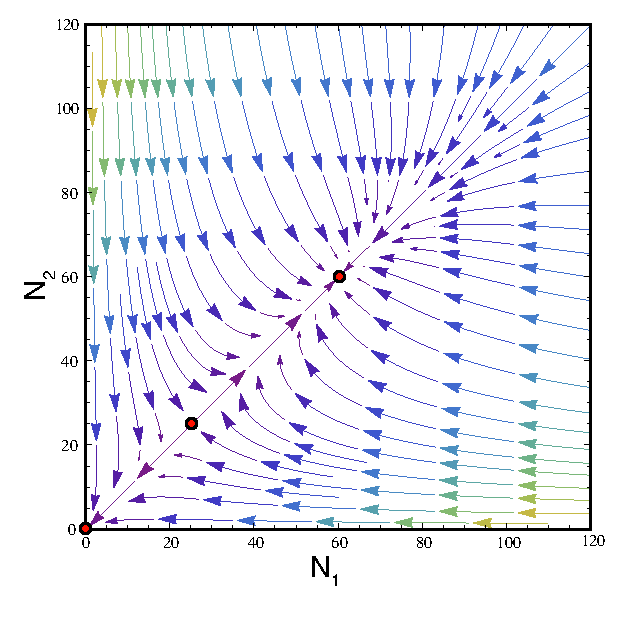
\includegraphics[scale=0.6]{DINAMICA_Figure2.eps}
\caption {Diagrama de flujo para la dinámica de ecuaciones de tipo II \ref{DINAMICA_eq_typeII}. Encontrar esta configuración requirió un ajuste de parámetros laborioso. Los valores empleados en este ejemplo son $r_1 = r_2 = -0.1$, $\alpha_1 = \alpha_2 = 0.001$, $a = 0.066$, $b = 0.2$ and $T_H = 1$.}
\label{DINAMICA_typeII}
\end{figure}

\subsection{La divisoria de la vida}
\label{watershed}

Llamaremos \textit{divisoria de la vida} al límte que separa las trayectorias que evolucionan hacia la capcidad máxima de población del sistema de las que terminan en su destrucción. En la imagen izquierda de la figura \ref{DINAMICA_diagram} es la curva que claramente delimita ambas cuencas. La divisoria incluye al \textit{saddle} no trivial $({N_1^p}^\bullet,{N_2^a}^\bullet)$, esto es la combinación mínima de poblaciones que garantiza la supervivencia. Su posición en el espacio de fases es importante porque determina la posición base de dicha curva y en consecuencia la fragilidad del sistema, que se expresa como la relación de áreas entre las dos cuencas de atracción. La distancia de este punto al máximo de poblaciones indica la resistencia ante perturbaciones externas. Si es muy pequeña, una ligera disminución del número de individuos, provocada por enfermedades, sequías o siniestros cualquier naturaleza puede llevar al sistema a la cuenca de destrucción. Por el contrario, si esta distancia es grande, la comunidad podrá recobrarse de estos eventos y crecer de nuevo hacia el máximo. Como los ciclos naturales suelen ser cíclicos, la combinación de poblaciones se moverá de manera habitual entre estos puntos, y un amplio rango dinámico facilita la permanencia en el tiempo. 

Para el sistema mínimo, de dos especies, las principales características de la divisoria se pueden encontrar analíticamente. Los puntos de la curva se corresponden a los pares de poblaciones $({N_1^p},{N_2^a})$ para los cuales la dinámica del sistema evoluciona exactamente sobre la curva y termina en el atractor $({N_1^p}^\bullet,{N_2^a}^\bullet)$. Sabemos que es un punto inestable y que la menor perturbación conducirá hacia uno u otro lado de la divisoria, pero conocer la expresión analítica de la curva supone un gran avance.  

Por definición, en $({N_1^p}^\bullet,{N_2^a}^\bullet)$ las tasas efectivas de crecimiento son nulas. Para llegar a este punto desde cualquier otro de la divisoria, las tasas de ambas especias deben ser de signo contrario y evolucionar en el tiempo de forma similar. Si las dos fueran del mismo signo, las trayetorias irían hacia la extinción (negativo) o hacia el máximo vital (positivo). 

Supongamos que el sistema se aproxima a $({N_1^p}^\bullet,{N_2^a}^\bullet)$, desde una posición inicial $({N_1^p}^0,{N_2^a}^0)$ pertencienta a la divisoria. Las tasas efectivas de crecimiento son:

\begin{align}
r_{ef,1}  = & \, A \, e^{-\gamma\, t} ,\nonumber\\  
r_{ef,2}  = & -B\, e^{-\gamma\, t} , 
\label{eq:coeffsreffs}
\end{align}
donde $A$, $B$ y $\gamma$ son constantes desconocidas por el momento. El sistema de ecuaciones \ref{eq:DINAMICA_dos_especies} se convierte en el siguiente:
\begin{align}
\frac{dN^p_{1}}{dt} & = N^p_{1} \, A \, e^{-\gamma \, t} , \nonumber \\
\frac{dN^a_{2}}{dt} & = -N^a_{2}\, B \, e^{-\gamma \, t} .
\label{eq:coeffsreffs_2}
\end{align}

Integrando ambas ecuaciones entre $t = 0$ e infinito  encontramos que:

\begin{align}
 \ln \frac{{N_1^p}^\bullet}{{N_{1}^p}^0} & = \frac{A}{\gamma} , \nonumber\\ 
 \ln \frac{{N_2^a}^\bullet}{{N_{2}^a}^0} & = - \frac{B}{\gamma} .
\label{eq:coeffsreffs_3}
\end{align}

Como el valor de $\gamma$ tiene que ser el mismo para ambas expresiones, obtenemos la condición que tienen que cumplir $({N_1^p}^0,{N_2^a}^0)$ para pertenecer a la divisoria:

\begin{align}
\frac{1}{B} \ln \left(\frac{{N_{2}^a}^\bullet}{{N_{2}^a}^0} \right) + \frac{1}{A} \ln \left(\frac{{N_1^p}^\bullet}{{N_1^p}^0} \right) = 0 ,
\label{eq:coeffsreffs_4}
\end{align}

Esto significa que la expresión funcional de la divisoria es una ley de potencia.

\begin{align}
{N_2^a}^0 = C\, ({N_1^p}^0)^\frac{-B}{A}. 
\label{eq:powerlaw}
\end{align}
Podemos despejar la constante $C$ teniendo en cuenta que la divisoria incluye el punto fijo $({N_1^p}^\bullet,{N_2^a}^\bullet)$, así que podemos escribir:

\begin{align}
C = {N_2^a}^\bullet / ({N_1^p}^\bullet)^\frac{-B}{A} .
\end{align}

Para encontrar el valor del exponente fraccionario $\frac{B}{A}$, debemos volver a la definición de ñas tasas de crecimiento efectivas $r_{ef,1}$ y $r_{ef,2}$. De acuerdo con las ecuaciones \eqref{eq:coeffsreffs}, en $t=0$ tenemos que:
 
\begin{align}
A = & \, r_{1}+ b_{12}\, {N_2^a}^0 - (\alpha_{1}+ c_{1} \, b_{12}\, {N_{2}^a}^0) \, {N_1^p}^0 , \nonumber\\
-B = &\, r_{2} + b_{21} \, {N_{1}^p}^0-(\alpha_{2}+ c_{2}\,  b_{21}\, {N_{1}^p}^0)\,  {N_{2}^a}^0 .
\label{eq:reffs_2especies}
\end{align}

Si sabemos que nuestro punto inicial era parte de la divisoria, podemos obtener el valor del exponente diviendo estas expresiones. Alternativamente, si necesitamos encontrar otros puntos de la divisoria que no sean $({N_1^p}^\bullet,{N_2^a}^\bullet)$, podemos dividir las expresiones anteriores y, usando la ecuación \ref{eq:coeffsreffs_3}, llegar a la siguiente ecuación implícita:

\begin{align}
\frac {\ln \left( \frac{{N_2^a}^\bullet}{{N_2^a}^0} \right)}{\ln \left( \frac{{N_1^p}^\bullet}{{N_1^p}^0} \right)} = \frac{( r_{2}+ b_{21}\, {N_1^p}^0) - (\alpha_{2}+ c_{2} \,  b_{21}\, {N_1^p}^0 ) \, {N_1^p}^0}{( r_{1}+ b_{12}\, {N_2^a}^0) - (\alpha_{1}+ c_{1} \, b_{12}\, {N_2^a}^0 ) \, {N_2^a}^0 } .
\label{eq:implicita_watershed}
\end{align}

Resolviendo esta ecuación de forma numérica podemos encontrar cualquier punto de la divisoria, y con ello obtenemos el valor del exponente $\frac{B}{A}$. La figura \ref{fig:powerlaw} muestra un ejemplo concreto de divisoria, y una comparación entre la curva definida por el sistema \ref{eq:powerlaw} y la ecuación implícita \eqref{eq:implicita_watershed}. Ambas se han resuelto por intergación numérica. Los puntos rojos se han encontrado haciendo un barrido del espacio de parámetros en una aproximación de \textit{fuerza bruta}, determinando el límite entre extinción y evolución hacia la capacidad máxima. La línea gris continua es la ley de potencia que se obtiene resolviendo las ecuaciones \eqref{eq:powerlaw} and \eqref{eq:implicita_watershed}

\begin{figure}[ht!]
\centering
\includegraphics[scale=0.5]{DINAMICA_Figure3.eps}
\caption {Divisoria de la vida para dos especies. En este caso, $\frac{B}{A}=1.2944,~{N_1^p}^\bullet=989,~{N_2^a}^\bullet=1232,~b_{12}=0.000041850,~c_{1}=0.00004,~\alpha_{1}=~0.000035,~r_1=-0.016,~b_{21}=0.00008750,~c_{2}=0.0001,~\alpha_{2}=0.000035,~r_2 =-0.02$.}
\label{fig:powerlaw}
\end{figure}

\subsection{Generalización con $n$ especies}
 
La generalización del análisis de establidad para un número cualquiera de especies es simple. Los puntos fijos del sistema \ref{eq:DINAMICA_modeloralphaconmut} incluyen la solución trivial de destrucción del sistema $(N_{i}^p,\cdots, N_{j}^a) = (0, \cdots,0)$, los puntos de extinción parcial cuando el mutualismo es facultativo para algunas especies y los puntos fijos no triviales $({N^{a}_{i}}^*,\cdots,{N^{p}_{j}}^*)$ en los que las tasas de crecimiento efectivas son nulas:
\begin{align}
r^{*}_{ef,i}  = (r_{i}+ \sum_{k=1}^{n_{p}}\,  b_{ik}\, {N^p_{k}}^*)- (\alpha_{i}+c_{i}\, \sum_{k=1}^{n_{p}} b_{ik}\, {N^{p}_k}^* )\, {N^{a}_{i}}^* = 0 \nonumber ,\\
r^{*}_{ef,j}  = (r_{j}+ \sum_{\ell=1}^{n_{a}} b_{j\ell}\, {N^{a}_{\ell}}^*)- (\alpha_{j}+c_{j}\, \sum_{\ell=1}^{n_{a}} b_{j\ell}\, {N^{a}_\ell}^* )\, {N^{p}_{j}}^* 
=0 ,
\label{eq:effrate2}
\end{align}
Estas son las expresiones para animales y plantas. Se puede reescribir el sistema como:

\begin{align}  
{N^{a}_{i}}^* = \frac{r_{i}+\sum_{k=1}^{n_{p}}b_{ik}\, {N^{p}_{k}}^*}{\alpha_{i}+c_{i}\,\sum_{k=1}^{n_{p}}{b_{ik}N^{p}_{k}}^*} = 
  \frac{r_{i}+r_{i}^{mut}}{\alpha_{i}+c_{i}\, r_{i}^{mut}} = 
  \frac{r_{i}^{*+}}{r_{i}^{*-}} , \nonumber\\
{N^{p}_{j}}^*=\frac{r_{j}+\sum_{\ell=1}^{n_{a}}b_{j\ell}\, {N^{a}_{\ell}}^*}{\alpha_{j}+c_{j}\,\sum_{\ell=1}^{n_{a}}{b_{j\ell}N^{a}_{\ell}}^*} =
  \frac{r_{j}+r_{j}^{mut}}{\alpha_{j}+c_{j}r_{j}^{mut}} =
  \frac{r_{j}^{*+}}{r_{j}^{*-}} .
\end{align}

Donde las tasas $r_{i}^{mut}$ representan el efecto del mutualismo sobre la especie $i$, mientras que las tasas $r^{*+}$ son las que incrementan el crecimento de la población y las $r^{*-}$ las que lo disminuyen vía competición intra especies. 

Las ecuaciones  \ref{eq:modeloralphaconmut} se pueden linealizar en torno a los puntos fijos. El jacobiano correspondiente tiene el mismo aspecto que el correpondiente al sistema mínimo de dos especies (ecuación \eqref{eq:J}), con términos negativos en la diagonal de la matriz y positivos o nulos fuera de ella. Para los puntos fijos no triviales se pueden escribir como (véase el Anexo \ref{DINAMICA_ANEXO_estabilidad}):
\begin{align}
\displaystyle & J_{ii}= - {N^{a}_{i}}^* \left(\alpha_{i} + c_{i} \,  \sum_{k=1}^{n_{p}} b_{ik} {N^{p}_{k}}^* \right), \nonumber\\
\displaystyle & J_{jj}= - {N^{p}_{j}}^* \left(\alpha_{j} + c_{j} \, \sum_{\ell=1}^{n_{a}} b_{j\ell}\, {N^{a}_{\ell}}^*\right).
\label{eq:Jii}
\end{align}
Los coeficientes fuera de la diagonal son:
\begin{align}
\displaystyle & J_{ij}={N^{a}_{i}}^* \, b_{ij}\, \left( 1-c_{i}\, {N^{a}_{i}}^*\right) 
\label{eq:Jij1}
\end{align}
para la interacción entre una especie animal $i$ y una planta $j$, y 
\begin{align}
\displaystyle & J_{ji}={N^{p}_{j}}^* \, b_{ji}\, \left( 1-c_{j}\, {N^{p}_{j}}^*\right)
\label{eq:Jij2}
\end{align}
para la correspondiente al sentido planta $j$ y animal $i$. Dada la invariancia de la traza de la matriz bajo un cambio de la base vectorial, la suma de autovalores de la matriz debe satisfacer la siguiente relación:
\begin{equation}
  \sum_{k}^{n_{a}+n_{p}} \lambda_{k}= - \left(\sum_{k}^{n_{a}+n_{p}} |J_{kk}| \right) .
  \stepcounter{equation}\tag{\theequation}\label{eq:sum_lambdas2}
\end{equation}
La traza es negativa, lo que significa que si hay autovalores positivos o nulos su efecto debe compensarse por otros autovalores negativos. En consecuencia, los puntos fijos no triviales pueden ser estables si todos los autovalores son negativos, o \textit{saddle} si al menos uno de ellos en positivo. No es posible que sean puramente inestables.

Otro extremo que hay que investigar es lo que sucede en caso de extinciones parciales. El efecto de la desaparición de algunas especies es reducir las dimensiones del sistema de ecuaciones \ref{eq:modeloralphaconmut}. Para hacerlo más simple, asumamos, por ejemplo, que la especie animal $e$ se extingue. Esto significa que los posibles puntos fijos del sistema deben incluir ahora ${N_e^a}^* = 0$. El colapso de $e$ puede provocar la extinción de algunas especies de plantas que se alimentaban con su polen, frutos o semillas, dependiendo del tipo de red. Estas extinciones pueden, a su vez, desencadenar la desaparición de especies animales que dependían de dichas plantas para su ciclo reproductivo. Este encadenamiento catastrófico es lo que se conoce como extinción en cascada. Aunque el fenómeno que produce la primera extinción sea externo y afecte a una sola especie, todas las demás se ven afectadas porque su dinámica está enlazada por el sistema de ecuaciones completo. Los nuevos puntos fijos no triviales se corresponden con los de extinción parcial del sistema original. La estabilidad de dichos puntos puede cambiar de manera sustancial con esta alteración de las condiciones. Los términos del jacobiano de las especies desaparecidas se convierten en $J_{ee} = r_e + \sum_{k =1}^{n_p }b_{ek}\,{N_k^p}^*$ en la diagonal y $J_{ej} = 0$ fuera de ella. Estos términos dejan de contribuir a los autovalores relevantes para la estabilidad del sistema. El resto de coeficientes del jacobiano se obtienen de las ecuaciones \ref{eq:Jii}, \ref{eq:Jij1}, y \ref{eq:Jij2} adaptadas a las especies supervivientes. Esto implica que los sumatorios de las ecuaciones \eqref{eq:Jii} ya no incluyen todas las especies y que los términos de la diagonal pueden estar más próximos a cero. La establidad de los nuevos puntos fijos puede variar dependiendo de los parámetros de las ecuaciones del modelo de dinámica de poblaciones de las especies supervivientes. En realidad, dependiendo de la configuración resultante de la comunidad reducida, el sistema puede ser más robusto ante extinciones parciales que antes. Esto puede explicar por qué las comunidades mutualistas adoptan configuraciones fuertemente anidadas, son el resultado por prueba y error en el tiempo de extinciones parciales y de la llegada de nuevas especies que alteran su dinámica.   

%\begin{figure}[h!]
%\centering
%\includegraphics[scale=1.1]{Figure4.eps}
%\caption {a) Mutualistic community with four species of plants and five species of pollinators. b) Simulation results with the population trends for the different species (each species is color-coded). Numerical solution shows that initial populations are below the \emph{extinction threshold}. In this scenario, the system tends to total extinction. The parameters of the simulation can be found in the \ref{DataTables} and table \ref{tab:experiment1}.}
%\label{fig:red_exper_stab1}
%\end{figure}

\section{Resultados}

Nunc posuere quam at lectus tristique eu ultrices augue venenatis. Vestibulum ante ipsum primis in faucibus orci luctus et ultrices posuere cubilia Curae; Aliquam erat volutpat. Vivamus sodales tortor eget quam adipiscing in vulputate ante ullamcorper. Sed eros ante, lacinia et sollicitudin et, aliquam sit amet augue. In hac habitasse platea dictumst.

\section{Conclusiones}

Nunc posuere quam at lectus tristique eu ultrices augue venenatis. Vestibulum ante ipsum primis in faucibus orci luctus et ultrices posuere cubilia Curae; Aliquam erat volutpat. Vivamus sodales tortor eget quam adipiscing in vulputate ante ullamcorper. Sed eros ante, lacinia et sollicitudin et, aliquam sit amet augue. In hac habitasse platea dictumst.

\section{Anexo: Análisis de la estabilidad en detalle}
\label{DINAMICA_ANEXO_estabilidad}

Para simplificar, prescindimos de los superíndices que representan las clases $animal$ y $planta$. 
El sitema de ecuaciones \ref{eq:DINAMICA_dos_especies} se desarrolla en serie de Taylor en la vecindad del punto singular ($N^{*}_{1}, N^{*}_{2}$) como  $N_{1}= N^{*}_1+\tilde{N}_{1}$ y $N_{2}= N^{*}_2+\tilde{N}_{2}$ \cite{murray1993mathematical}:

\begin{equation}
\begin{array}{lcr}
\displaystyle \frac{d\tilde{N}_{1}}{dt} = r_{1}+ b_{12}(N^{*}_2+\tilde{N}_{2})-(\alpha_{1}+ c_{1} b_{12} (N^{*}_2+\tilde{N}_{2}))( N^{*}_1+\tilde{N}_{1})\nonumber\\
\\
\displaystyle \frac{d\tilde{N}_{2}}{dt} = r_{2}+ b_{21}( N^{*}_1+\tilde{N}_{1})-(\alpha_{2}+ c_{2} b_{21}(N^{*}_1+\tilde{N}_{1}))(N^{*}_2+\tilde{N}_{2}) 
\stepcounter{equation}\tag{\theequation}\label{eq:effrateTaylor}
\end{array}
\end{equation}

\noindent y quedándonos solo con los términos de primer orden:

\begin{equation}
\begin{array}{lcr}
\displaystyle \frac{d\tilde{N}_{1}}{dt}= \tilde{N}_{2}( b_{12} - c_{1} b_{12}\, N^{*}_1)-\tilde{N}_{1}(\alpha_{1}+ c_{1} b_{12} \, N^{*}_2) \equiv f_{1}(\tilde{N}_{1},\tilde{N}_{2}) \nonumber\\
\\
\displaystyle \frac{d\tilde{N}_{2}}{dt} = \tilde{N}_{1}( b_{21} - c_{2} b_{21}\, N^{*}_2)-\tilde{N}_{2}(\alpha_{2}+ c_{2} b_{21} \, N^{*}_1) \equiv f_{2}(\tilde{N}_{1},\tilde{N}_{2})
\stepcounter{equation}\tag{\theequation}\label{eq:effrateTaylor2}
\end{array}
\end{equation}

\noindent Los términos del jacobiano son:

\begin{equation}
\begin{array}{l}
J_{11}= \frac{\partial f_{1}}{\partial \tilde{N}_{1}} =- N^{*}_{1}\left(\alpha_{1}+ c_{1} b_{12} \, N^{*}_2\right)  \\
\\
J_{12}= \frac{\partial f_{1}}{\partial \tilde{N}_{2}} = N^{*}_{1}b_{12}\left(1 - c_{1}\, N^{*}_1\right) \\
\\
J_{21}= \frac{\partial f_{2}}{\partial \tilde{N}_{1}} = N^{*}_{2}b_{21} \left(1 - c_{2}\, N^{*}_2\right) \\
\\
J_{22}= \frac{\partial f_{2}}{\partial \tilde{N}_{2}} = - N^{*}_{2}\left(\alpha_{2}+ c_{2} b_{21}\,N^{*}_{1}\right)
\end{array}
\stepcounter{equation}\tag{\theequation}\label{eq:J11}
\end{equation}

\noindent que puede reescribirse en términos de los coeficientes positivos $J_{ij}$ como:

\begin{equation*}
J = \left(
\begin{array}{rr}
-J_{11} & J_{12} \\ J_{21} & -J_{22}
\end{array}
\right)
\end{equation*}

\noindent Los autovalores $\lambda_{1,2}$ se obtienen de
\begin{equation}
\lvert J - \lambda I \rvert =0
\stepcounter{equation}\tag{\theequation}\label{eq:lambda0App}
\end{equation}

\noindent cuyas soluciones son
\begin{equation}
\begin{array}{lcl}
\lambda _{1,2}=\frac{1}{2}\left(tr(J)\pm \sqrt{tr^{2}(J)-4\,\mathrm{Det}(J)}\right)\\ =
\frac{1}{2}\left(-\left(J_{11}+J_{22}\right)\pm \sqrt{\left(J_{11}+J_{22}\right)^{2}-4\,\mathrm{Det}(J)}\right)\\  =
\frac{1}{2}\left(-\left(J_{11}+J_{22}\right)\pm \sqrt{\left(J_{11}-J_{22}\right)^{2} +4 \,\left( J_{12}J_{21} \right) }\right)
\end{array}
\stepcounter{equation}\tag{\theequation}\label{eq:lambda12}
\end{equation}

\noindent La última expresión indica que los dos autovalores son reales. Además, satisfacen la siguiente condición:

\begin{equation}
\prod_{k}\lambda_{k}=\mathrm{Det}(J)
\end{equation}

\noindent por tanto el punto singular será un \textit{saddle} cuando se cumpla que  $\mathrm{Det}(J)<0$. Expandiendo el determinante del jacobiano obtenemos la condición de existencia del \textit{saddle}:

\begin{equation}
1-c_{1}N^{*}_{1}-c_{2}N^{*}_{2} >0
\end{equation}

Las extinciones parciales son también puntos singulares, y corresponden a $N^{*}_{1,2} = 0$. Para simplificar, escribimos solo las ecuaciones del punto singular  ($N^{*}_{1}=r_{1}/\alpha_{1},N^{*}_{2}=0$). Expandiendo en serie de Taylor en torno a él, el sistema de ecuaciones se convierte en:

\begin{equation}
\begin{array}{ll}
\displaystyle \frac{d\tilde{N}_{1}}{dt} = & r_{1} N^{*}_{1}-\alpha_{1}N^{*2}_{1}+r_{1}\tilde{N}_{1}+ b_{12}\tilde{N}_{2}N^{*}_1-2\alpha_{1}N^{*}_1\tilde{N}_{1} + \\
\, & - c_{1} b_{12}\tilde{N}_{2}N^{*2}_1\nonumber\\
\displaystyle \frac{d\tilde{N}_{2}}{dt} = & r_{2}\tilde{N_{2}}+ b_{21} N^{*}_1\tilde{N_{2}} 
\end{array}
\label{eq:effrateTaylorN2=0}
\end{equation}

\noindent El jacobiano es ahora:

\begin{equation*}
J = \left(
\begin{array}{rr}
-r_{1} & b_{12}N^{*}_{1}\left(1-c_{1}N^{*}_{1}\right) \\
0 & r_{2}+b_{21}N^{*}_{1}
\end{array}
\right)
\end{equation*}

Los autovalores son los términos de la diagonal. Este punto será estable si se cumple que $r_{1}>0$ y que $r_{2}<-b_{21}r_{1}/\alpha_{1}$. La solución simétrica es ($N^{*}_{1}=0,N^{*}_{2}=r_{2}/\alpha_{2}$) y será estable si  $r_{2}>0$ y $r_{1}<-b_{12}r_{2}/\alpha_{2}$. La generalización para $n_{a} + n_{p}$ especies es:
 
\begin{align}
\frac{dN_{i}}{dt} = \left( r_{i}+ \sum_{j=1}^{n_{a}} b_{ij}N_{j}\right)N_{i} - \left(\alpha_{i}+ c_{i} \sum_{j=1}^{n_{a}} b_{ij}N_{j} \right) N^{2}_{i} \nonumber\\ 
\frac{dN_{j}}{dt} = \left( r_{j}+ \sum_{i=1}^{n_{p}} b_{ji}N_{i}\right)N_{j} - \left(\alpha_{j}+ c_{j} \sum_{i=1}^{n_{p}} b_{ji} N_{i} \right) N^{2}_{j} 
\stepcounter{equation}\tag{\theequation}\label{eq:N_especies}
\end{align}

\noindent donde el subíndice $i$ se extiende para todas las especies de plantas y el $j$ para todas las de animales.

Los puntos fijos de este sistema son la solución trivial de destrucción completa de la comunidad ($N_{i=1\cdots n_{p}}=0, N_{j=1\cdots n_{a}}=0$), y las soluciones para las que las tasas de crecimiento efectivas se anulan: 

\begin{equation}
\begin{array}{lcr}
\displaystyle r^{*}_{ef,i} =\left(r_{i}+ \sum_{j=1}^{n_{a}} b_{ij}N^{*}_{j}\right)- \left(\alpha_{i}+c_{i}\sum_{j=1}^{n_{a}} b_{ij}N^{*}_j\right)N^{*}_{i}
=0 \nonumber\\
\displaystyle r^{*}_{ef,j} = \left(r_{j}+ \sum_{i=1}^{n_{p}} b_{ji}N^{*}_{i}\right)- \left(\alpha_{j}+c_{j}\sum_{i=1}^{n_{p}} b_{ji}N^{*}_i\right)N^{*}_{j} 
=0 
\stepcounter{equation}\tag{\theequation}\label{eq:effrateN}
\end{array}
\end{equation}

\noindent que pueden reescribirse como un conjunto de ecuaciones implícitas.

\begin{eqnarray}
\begin{array}{lcc}
  N^{*}_{i}=\frac{r_{i}+\sum_{j=1}^{n_{a}}b_{ij}N^{*}_{j}}{\alpha_{i}+c_{i}\sum_{i=1}^{n_{p}}b_{ij}N^{*}_{j}} = 
  \frac{r_{i}+r_{i}^{Mut}}{\alpha_{i}+c_{i}r_{i}^{Mut}} = 
  \frac{r_{i}^{*+}}{r_{i}^{*-}}  \nonumber\\
  \\
  N^{*}_{j}=\frac{r_{j}+\sum_{i=1}^{n_{p}}b_{ji}N^{*}_{i}}{\alpha_{j}+c_{j}\sum_{i=1}^{n_{a}}b_{ij}N^{*}_{i}} =
  \frac{r_{j}+r_{j}^{Mut}}{\alpha_{j}+c_{j}r_{j}^{Mut}} =
  \frac{r_{j}^{*+}}{r_{j}^{*-}}
  \end{array}
\end{eqnarray} 
 
\noindent donde las tasas $r^{*+}$ y $r^{*-}$ representan el efecto positivo sobre el crecimiento y el negativo, respectivamente. El sistema \ref{eq:N_especies} puede también desarrollarse en torno al punto singular:

\begin{equation}
\begin{array}{lcl}
\textstyle \frac{dN_{i}}{dt}=r_{i}+\sum\limits_{j=1}^{n_{a}}b_{ij}(N^{*}_{j}+\tilde{N}_{j})- (\alpha_{i}+c_{i}\sum\limits_{j=1}^{n_{a}}b_{ij}(N^{*}_j+\tilde{N}_{j}))(N^{*}_i+\tilde{N}_{i}) \nonumber\\
\textstyle \frac{dN_{j}}{dt}=r_{j}+\sum\limits_{i=1}^{n_{p}}b_{ji}(N^{*}_{i}+\tilde{N}_{i})-(\alpha_{j}+c_{j}\sum\limits_{i=1}^{n_{p}}b_{ji}(N^{*}_i+\tilde{N}_{i}))(N^{*}_j+\tilde{N}_{j}) 
\stepcounter{equation}\tag{\theequation}\label{eq:effrateTaylorN}
\end{array}
\end{equation}

\noindent donde el subíndice $i$ corresponde a las plantas y el $j$ a los animales. El conjunto de $n_{a} + n_{p}$ ecuaciones se reescribe en términos lineales como:

\begin{align}
\begin{array}{lcl}
\displaystyle \frac{dN_{i}}{dt} = \sum_{j=1}^{n_{a}} \tilde{N}_{j} \left(  b_{ij} - c_{i} b_{ij}\, N^{*}_i\right) - \tilde{N}_{i}(\alpha_{i}+ c_{i} \sum_{j=1}^{n_{a}} b_{ij} \, N^{*}_{j})\nonumber\\
\displaystyle \frac{dN_{j}}{dt} = \sum_{i=1}^{n_{p}} \tilde{N}_{i} \left( b_{ji} - c_{j} b_{ji}\, N^{*}_j\right) - \tilde{N}_{j}(\alpha_{j}+ c_{j} \sum_{i=1}^{n_{p}} b_{ji} \, N^{*}_{i})\stepcounter{equation}\tag{\theequation}\label{eq:effrateTaylor2N}
\end{array}
\end{align}

Los coeficientes de $\tilde{N}_{i,j}$ son los términos del jacobiano. Los valores absolutos de los elementos de la diagonal, para cualquier especie $i$ de plantas, $j$ de animales son:

\begin{align}
\displaystyle & J_{ii}=N^{*}_{i}\left(\alpha_{i} + c_{i} \sum_{j=1}^{n_{a}} b_{ij} N^{*}_{j}\right) \nonumber\\
\displaystyle & J_{jj}=N^{*}_{j}\left(\alpha_{j} + c_{j} \sum_{i=1}^{n_{p}} b_{ji} N^{*}_{i}\right)
\label{eq:Jii2}
\end{align}

\noindent y los términos fuera de la diagonal:

\begin{align}
\displaystyle & J_{ij}=N^{*}_{i}b_{ij}\left( 1-c_{i}N^{*}_{i}\right)\nonumber\\
\displaystyle & J_{ji}=N^{*}_{j}b_{ji}\left( 1-c_{j}N^{*}_{j}\right)
\label{eq:Jij}
\end{align}

\noindent Como resultado el jacobiano queda así:

\begin{equation*}
J=\left(
   \begin{array}{ccccc}
      \ddots  & \cdots & \cdots & \cdots & \cdots \\
      \cdots  & -J_{ii} & \cdots & J_{ij} & \cdots \\
      \vdots  & \vdots & \ddots  & \vdots & \vdots  \\
      \cdots  & J_{ji} & \cdots & -J_{jj} & \cdots \\
      \cdots  & \cdots & \cdots & \cdots  & \ddots
   \end{array}
\right)
\end{equation*}

\noindent con todos los términos de la diagonal negativos y el resto positivos. La suma de los autovalores satisface la sigiente igualdad:

\begin{equation}
  \sum_{k}^{n_{a}+n_{p}} \lambda_{k}= -\left(\sum_{k}^{n_{a}+n_{p}} J_{kk}\right)
  \stepcounter{equation}\tag{\theequation}\label{eq:sum_lambdas}
\end{equation}

Esto significa que no todos los autovalores son positivos y que por tanto el punto singular no es asintóticamente inestable. Por otra parte, los autovalores no pueden ser complejos porque todos los coeficientes fuera de la diagonal del jacobiano son positivos o nulos, por tanto los puntos fijos deben ser estables o \textit{saddle}.